\documentclass[10pt,conference]{IEEEtran}
\IEEEoverridecommandlockouts

\usepackage{cite}
\usepackage{amsmath,amssymb,amsfonts}
\usepackage{algorithmic}
\usepackage{graphicx}
\usepackage{textcomp}
\usepackage{xcolor}
\usepackage{subfig}
\usepackage{listings}
\usepackage[mathscr]{euscript}
\usepackage{amsmath}


% \usepackage{subcaption}
\lstset{numbers=left,stepnumber=1,basicstyle=\footnotesize\ttfamily}
\def\BibTeX{{\rm B\kern-.05em{\sc i\kern-.025em b}\kern-.08em
T\kern-.1667em\lower.7ex\hbox{E}\kern-.125emX}}
\def\code#1{\texttt{#1}}
\def\dist{\mathcal{D}}
\def\hypspace{\mathcal{H}}
\DeclareMathOperator*{\argmax}{argmax}
\DeclareMathOperator*{\argmin}{argmin}

\makeatletter
\def\endthebibliography{%
  \def\@noitemerr{\@latex@warning{Empty `thebibliography' environment}}%
  \endlist
}
\makeatother

\begin{document}

\title{Probably Approximately Correct Learning - An Introduction in the Finite Case\\}

\author{\IEEEauthorblockN{Kevin de Haan}
  \IEEEauthorblockA{ \\
    Edmonton, Canada\\
  Email: kdehaan@ualberta.ca}
}

\maketitle

\begin{abstract}
  Probably Approximately Correct (PAC) learning is a tool that was first introduced in 1984 by Valiant in order to bridge the gap between computability theory and machine learning\cite{valiant}. In doing so, Valiant introduced the concept of learnability to a wider group of computer scientists interested in algorithmic efficiency and leading to the combined field of computational learning theory\cite{haussler:}.
\end{abstract}

\begin{IEEEkeywords}
  PAC; Learning Theory; Computability Theory; Computational Learning Theory
\end{IEEEkeywords}


\section{Introduction}
  The Probably Approximately Correct (hereafter PAC) learning framework, first introduced by Valiant \cite{valiant}, is a method for determining the learnability of a problem for a machine classifier. In other words, using the PAC learning framework one can estimate whether a learning classifier will be able to output an approximately correct prediction, and under what conditions the classifier is able to operate. If a concept is known to be PAC-learnable, it means that the learning algorithm must be able to operate in polynomial time \cite{haussler:}, and additionally provides an upper bound on the volume of training samples provided to the classifier in order to produce an acceptable prediction \cite{haussler:}. It can also be useful to prove that a target is not PAC-learnable, for example in the case of a cryptographic function \cite{haussler:}.

\section{Deriving the Key Points of PAC Learning}
  \subsection{Terminology}
  PAC and indeed learning theory as a whole has some terminology that varies from traditional machine learning notation. All non-trivial symbols used in this paper can be found in the following list:
  \begin{itemize}
    \item $X$: the domain space
    \item $Y$: the label set space
    \item $f$: the mapping function between domain set space to label set space, $f: X \rightarrow Y$. Unknowable in its entirety.
    \item $\dist$: the data distribution over $X$. Unknowable in its entirety.
    \item $S$: a sample taken from $\dist$
    \item $h$: a hypothesis, also referred to as a $model$. A prediction of the real mapping function $f$
    \item $\hypspace$: a finite hypothesis space
    \item $L$: a $learner$, the algorithm or device that produces a hypothesis $h$
    \item \emph{risk}: used interchangeably with 'error rate'
    \item $\delta$: the probability of getting a nonrepresentative sample $S$ from $\dist$
  \end{itemize} 
  \subsection{Background: Empirical Risk Minimization}
  To properly understand the theory behind PAC, it is valuable to have an understanding of Empirical Risk Minimization (hereafter ERM). The fundamental theory behind ERM is that given some $h \in \hypspace$ produced from the training set $S$, there will be some error between $h_S$ and the real $f$, demonstrated in equation \ref{trueerror}. The true error is equal to the probability of sampling $x$ from $\dist$ such that prediction of $h$ is different from that of $f$\cite{shais}.

  \begin{equation}
    \label{trueerror}
    L_{\dist, f}(h) = \dist(\{x : h(x) \neq f(x)\})
  \end{equation}

  However, because $\dist$ and $f$ are unknown, the full error calculation cannot simply be evaluated by the learner $L$\cite{shais}. The next best thing is to determine the \emph{training error}, the error encountered by the classifier in the process of training (equation \ref{trainingerror})\cite{shais}. The training error is equal to the real number of times that the prediction from $h$ has been different from the real value in $y$, divided by the number of samples $m$. This is also referred to as the \emph{empirical error} or \emph{empirical risk} interchangeably\cite{shais}.

  \begin{equation}
    \label{trainingerror}
    L_S(h) = \frac{|\{i \in [m] : h(x_i) \neq y_i\}|}{m}, [m] = \{1, ..., m\}
  \end{equation}

  In contrast to the real error (or \emph{actual risk}) the value of empirical risk is available to the learner and is therefore an obvious choice for minimization - hence, the goal of \emph{empirical risk minimization} defined in eq. \ref{erm} \cite{shais}.

  \begin{equation}
    \label{erm}
    h_S \in \argmin_{h \in \hypspace} L_S(h)
  \end{equation}

  Now, what can be done with this empirical risk? By using the \emph{realizability assumption} and the \emph{i.i.d. assumption}, we can establish an upper bound on the error of the model.

  \subsubsection{\textbf{The Realizability Assumption}} 
    "There exists $h^* \in \hypspace$ s.t. $L_{(\dist, f)}(h^*) = 0$"\cite{shais}. This implies that given enough sets of samples $S$ from the distribution $\dist$, there exists some $S$ such that $L_S(h^*) = 0$ with probability 1. This in turn suggests that for every ERM domain and hypothesis there exists an optimal $h_S$ such that $L_S(h_S) = 0$. However, this only applies to the empirical risk - what about the real risk? And what about overfitting? This leads us to the next step:
  \subsubsection{\textbf{The i.i.d. Assumption}} 
    "Examples in the training set are independently and identically distributed (i.i.d.) according to the distribution" $\dist$\cite{shais}. This means that every element $x_i \in S$ is sampled according to $\dist$ and in turn labelled according to $f$, denoted by the term $S \sim \dist^m$ such that $m$ is the size of $S$\cite{shais}. The key feature of this assumption is that as $m$ increases, the likelihood that $S$ is properly representing $\dist$ (and that $h_S$ reflects $f$) also increases\cite{shais}.
  
    From these two assumptions, we can establish that there is some chance less than 1 for any properly sampled $S$ to be a misrepresentation of $\dist$, labelled $\delta$, and consequentially we are able to formally name $(1-\delta)$ as the \emph{confidence parameter} of a prediction\cite{shais}.

    In addition to describing the chance for the sample $S$ to be nonrepresentative, we can also choose a value to describe the quality of the hypothesis $h$. This is the \emph{accuracy parameter} $\epsilon$, the threshold of error or risk above which the model is considered to be to inaccurate to be useful\cite{shais}. I.e, a risk $L_{(\dist, f)}(h_S) > \epsilon$ is a failure, while $L_{(\dist, f)}(h_S) \leq \epsilon$ is \textbf{\emph{approximately correct}}.


\section{Conclusion and Critical Analysis}
  
  % \begin{figure}
  %   \centering
  %   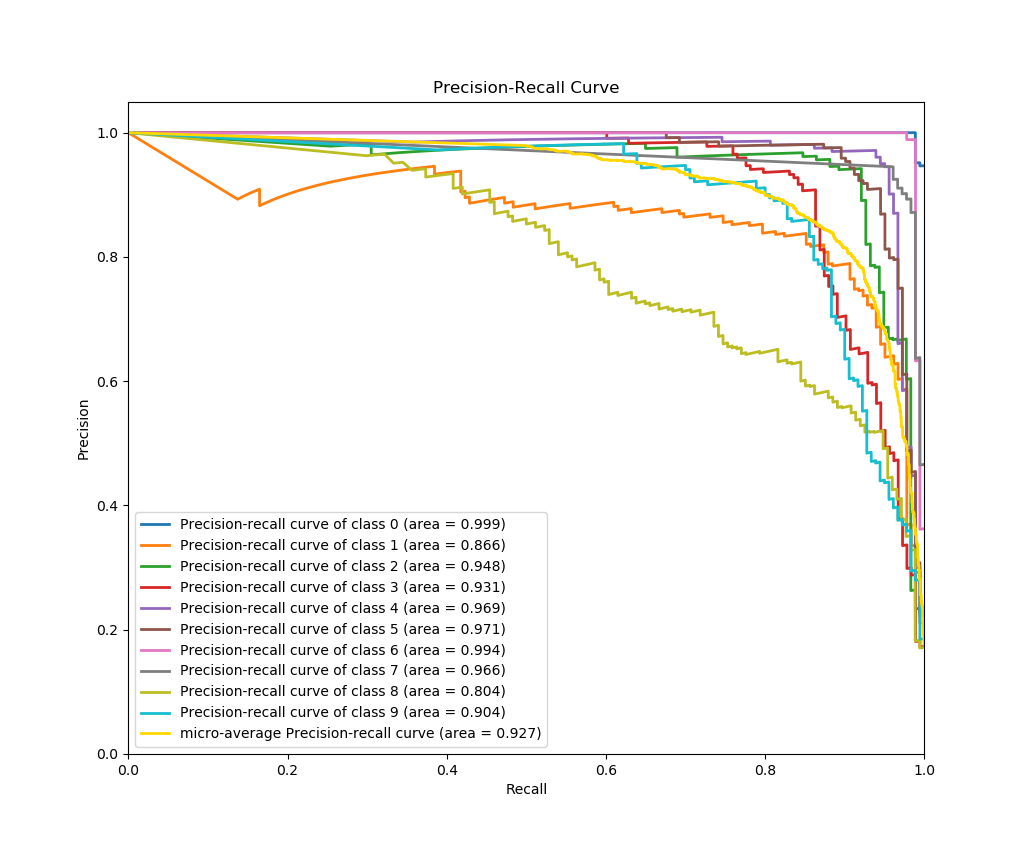
\includegraphics[width=0.4\textwidth]{figures/example.png}
  %   \caption{Example Figure}
  %   \label{samplefig}
  % \end{figure}
\nocite{*}
\bibliography{bib/refs}
\bibliographystyle{IEEEtran}


\vspace{12pt}

\end{document}